\documentclass[10pt,a4paper]{article}
\usepackage[T1]{fontenc}
\usepackage[utf8]{inputenc}
\usepackage{mathpazo}
\usepackage[margin=22mm,top=22mm,bottom=24mm]{geometry}
\usepackage{microtype,booktabs,graphicx,xcolor,amsmath,float,caption,subcaption,tabularx,enumitem,listings,tikz}
\usetikzlibrary{arrows.meta,positioning}
\usepackage[colorlinks=true,linkcolor=accent,urlcolor=accent,citecolor=accent]{hyperref}
\definecolor{accent}{HTML}{1F5FA8}
\definecolor{codebg}{HTML}{F5F6F8}
\definecolor{boxbg}{HTML}{EEF4FB}
\definecolor{warnbg}{HTML}{FDF3E4}
\captionsetup{font=small,labelfont=bf,skip=6pt}
\setlist{itemsep=1pt,topsep=3pt,leftmargin=1.4em}
\setlength{\parskip}{4pt}\setlength{\parindent}{0pt}
\lstset{language=Python,basicstyle=\ttfamily\scriptsize,backgroundcolor=\color{codebg},frame=single,rulecolor=\color{codebg},
  keywordstyle=\color{accent}\bfseries,commentstyle=\color{black!55},showstringspaces=false,columns=fullflexible,keepspaces=true,
  xleftmargin=2pt,xrightmargin=2pt,aboveskip=6pt,belowskip=4pt,breaklines=true,captionpos=b}
\newcommand{\takeaway}[1]{\par\smallskip\noindent\colorbox{boxbg}{\parbox{\dimexpr\linewidth-2\fboxsep}{\small\textbf{Takeaway.} #1}}\par\smallskip}
\newcommand{\caution}[1]{\par\smallskip\noindent\colorbox{warnbg}{\parbox{\dimexpr\linewidth-2\fboxsep}{\small\textbf{Caution.} #1}}\par\smallskip}
\newcommand{\algo}[1]{\texttt{#1}}
\newcommand{\figs}{../notes/figs}

\title{\vspace{-8mm}\textbf{Making the UREX Tread-Depth Software Robust:\\ A Benchmark Study of Ten Algorithm Families\\ on Simulated and Real Laser-Line Images}}
\author{UREX project team \\ \small Technical report \,\textperiodcentered\, 12 November 2026 \,\textperiodcentered\, code: \texttt{github.com/Advait-B/urex}, branches \texttt{research/*}}
\date{}

\begin{document}
\maketitle
\vspace{-6mm}
\begin{abstract}
\noindent UREX is a handheld device that measures bus tyre tread depth by laser triangulation: a camera looks down at
the tread, a line laser strikes it at $35^\circ$, and the line shifts by about 2\,px for every millimetre of groove
depth. Our existing software works on good photos but reports a depth on most bad ones. We built a ray-traced
simulator of the printed holder and a benchmark with exact ground truth (five test sets, 800 frames), and used it,
together with 86 real hand-held photos, to compare ten families of algorithms: sub-pixel peak detectors,
dynamic-programming line tracking, a small U-Net, a learned candidate classifier, a robust depth stage, calibration
models, a quality gate, laser on/off subtraction, an end-to-end network, and a combination. The best single-frame
pipeline is almost entirely classical: Viterbi line tracking, a depth stage that fits the tread in millimetres and
clusters the groove floor, and two logistic-regression gates that can ask for a retake. Under simulated bad
conditions it reduces the mean depth error from 1.52 to 0.25\,mm, gross errors ($>1$\,mm) from 36\,\% to 2.7\,\%, while
answering 89\,\% of presses; across the three hardest sets it passes none of 41 illegal tyres where the baseline
passes 9; on real photos it stops reporting
depths on frames with no laser (cross-validated: 0 of 55) and agrees with the reference depths to about one pixel.
An independent audit reproduced every number exactly and found no training on test data. Networks that replace the geometry scored well on data like their training set and failed on other units and on
real photos. Laser on/off subtraction, which the firmware can already capture, would roughly halve the remaining error in simulation. A
preliminary hand-held test on a tyre of about 9\,mm gave repeatable pixel readings but millimetre estimates 2.4--4.2
times too large, because the camera--laser geometry was not fixed. Real-world accuracy is therefore still unmeasured;
calibrated measurements with the printed holder are the most valuable next step.
\end{abstract}

\section{Introduction}

SMRT inspects more than 1{,}000 buses, and each inspection includes measuring tyre tread depth by hand at several
points on every tyre. The UREX device replaces the hand gauge with a handheld optical head: a camera looks straight
down at the tread and a green line laser strikes the tread at an angle. Where the rubber is lower (inside a groove)
the laser line appears shifted in the image, and the size of the shift gives the depth. This is \emph{laser
triangulation}.

The software has one job: turn one greyscale image into a groove depth in millimetres, and a PASS / FAIL against the
1.6\,mm legal limit. The pipeline we had on 12 November (the \emph{baseline}) does this in three steps:
(1) find the laser line with a Steger ridge detector, (2) fit the tread surface and read how far the line drops
inside each groove, (3) convert pixels to millimetres with a calibration. It works on good photos, but it also
reports a depth on most \emph{bad} photos, and it has never been tested against known answers.

This report asks a practical question: \textbf{which algorithms actually make the software more robust, and by how
much?} To answer it we built a simulator of the printed holder, a fixed benchmark with exact ground truth, and then
tried ten families of algorithms, each on its own git branch, all scored by the same harness on the same frames and
on the 86 real photos taken between 8 and 30 October.

\paragraph{Contributions.}
\begin{itemize}
\item A ray-traced simulator of the Rev\,A holder on a tyre, with exact truth for the laser line and every groove
      (Section~\ref{sec:sim}).
\item A benchmark of five simulated test sets plus the real photos, and a scorer that rewards an algorithm for
      saying ``retake the photo'' instead of guessing (Section~\ref{sec:bench}).
\item A like-for-like evaluation of ten algorithm families: sub-pixel peak detectors, dynamic-programming line
      tracking, a small U-Net, a candidate classifier, a robust depth stage, calibration models, a quality gate,
      laser on/off subtraction, an end-to-end network, and a combined stack (Sections~\ref{sec:algos}--\ref{sec:stack}).
\item An independent audit of the numbers (Section~\ref{sec:audit}), and an honest list of what the simulator and the
      real photos can and cannot tell us (Section~\ref{sec:validity}).
\end{itemize}

\section{The device and the measurement}\label{sec:device}

Figure~\ref{fig:geometry} shows the geometry of the printed holder. The holder's feet rest on the tread, so the
camera height and the laser angle are fixed. The numbers used throughout are in Table~\ref{tab:device}.

\begin{figure}[H]
\centering
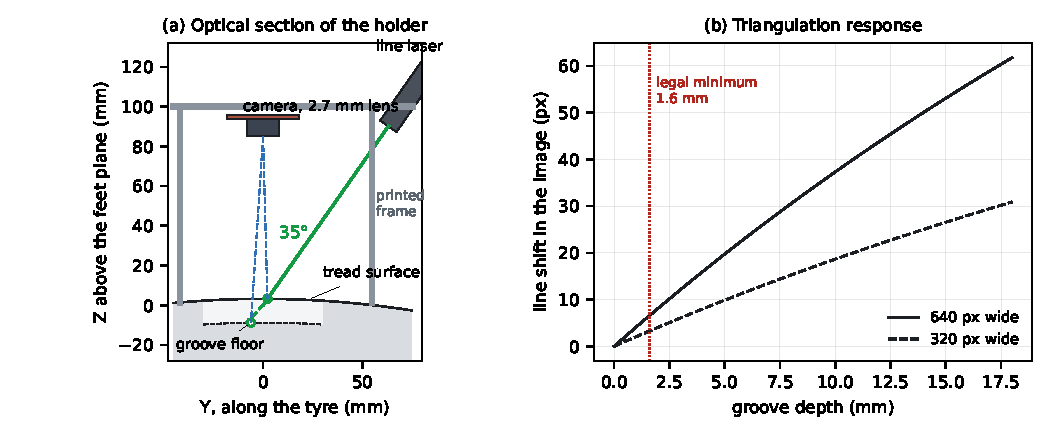
\includegraphics[width=0.86\linewidth]{figs/fig_geometry.pdf}
\caption{Side view of the holder on a tyre. The camera looks straight down; the laser sheet arrives at
$35^\circ$. A groove floor lies lower than the tread, so the laser meets it further along, and the camera sees the
line shifted.}
\label{fig:geometry}
\end{figure}

\begin{table}[H]
\centering\small
\caption{Device constants (holder Rev\,A, OV5640 camera with a 2.7\,mm lens).}\label{tab:device}
\begin{tabular}{@{}lll@{}}
\toprule
Quantity & Value & Comment \\
\midrule
Camera height above the feet plane & 85\,mm & lens front, looking straight down \\
Focal length & 2.7\,mm (235\,px at 320\,px image width) & horizontal field of view $68^\circ$ \\
Laser angle $\theta$ & $35^\circ$ from vertical & $110^\circ$ fan across the tread \\
Tyre radius / crown height & 480\,mm / 3.2\,mm above the feet plane & bus tyre between the feet \\
Image used by the algorithms & $320\times240$ greyscale & down-sampled; real photos are $240\times320$ \\
Legal limit & 1.6\,mm & PASS only if every groove is deeper \\
\bottomrule
\end{tabular}
\end{table}

\paragraph{How a depth becomes a pixel shift.} Let $H$ be the distance from the lens to the tread surface
(about 82\,mm) and $f$ the focal length in pixels. A groove of depth $d$ moves the laser spot sideways by
$d\tan\theta$ on the tyre and puts it $d$ further from the camera, so the line moves in the image by
\begin{equation}
\Delta v \;=\; \frac{f\, d \tan\theta}{H + d}
\qquad\Longrightarrow\qquad
d \;=\; \frac{H\,\Delta v}{f\tan\theta - \Delta v}.
\label{eq:tri}
\end{equation}
With our numbers this is about \textbf{2.1\,px of shift per millimetre of depth}, and about 2.9\,px per millimetre
across the tread. Two consequences follow, and they explain most of this report:
\begin{itemize}
\item An error of only 0.2\,px in locating the line is already 0.1\,mm of depth. Sub-pixel accuracy matters.
\item One wrong decision about \emph{which bright thing is the laser} (a glint, a wet patch, the edge of a thick
      saturated line) is an error of many millimetres. Robustness matters more.
\end{itemize}
In practice we do not use Eq.~\eqref{eq:tri} directly. A calibration (Section~\ref{sec:calib}) maps each image
position to a height, which also absorbs lens distortion and assembly tolerances.

\section{Method: simulator, benchmark and scorer}

\subsection{Simulator}\label{sec:sim}

Real photos have no ground truth: nobody measured those grooves with a gauge. So we wrote a simulator,
\texttt{research/sim/holder\_sim.py}, that renders what the camera in the holder would see. It builds a tyre
surface (radius 480\,mm, a gentle crown, circumferential grooves with sloped walls and optional rounded floors),
traces 2{,}400 laser rays to the first surface they hit, checks that the camera can see each hit, and renders the
line with realistic blur, sensor noise, lens distortion and JPEG compression. Because the scene is known, every
frame comes with the exact sub-pixel laser line and the exact depth of every groove, plus a laser-off frame of the
same scene.

The simulator can also make conditions worse on purpose: rocking of the holder, sunlight, wet glints, stones in
grooves, zig-zag grooves, mud that hides part of the line, paint, a dim or a saturated laser. Figure~\ref{fig:simreal}
compares simulated frames with real photos.

\begin{figure}[H]
\centering
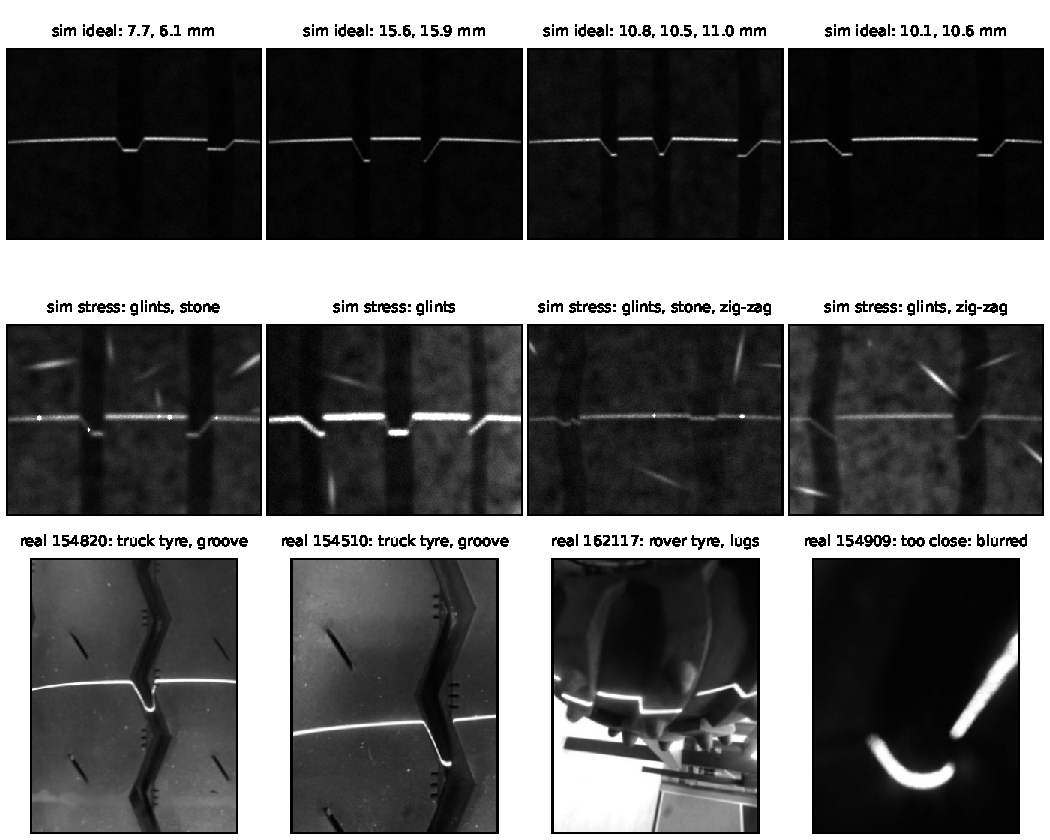
\includegraphics[width=\linewidth]{figs/fig_sim_vs_real.pdf}
\caption{Simulated frames (holder locked in place) next to real photos (hand-held, October). The simulated ``ideal''
line is thin and level; real lines are thicker, often saturated, and can sit anywhere in the frame.}
\label{fig:simreal}
\end{figure}

\subsection{Test sets}\label{sec:bench}

\begin{table}[H]
\centering\small
\caption{The benchmark. Algorithms may train or tune only on \texttt{train}; all other sets are for testing.}\label{tab:sets}
\begin{tabularx}{\linewidth}{@{}llX@{}}
\toprule
Set & Frames & What it represents \\
\midrule
\texttt{ideal} & 150 & Holder locked on a clean tyre in shade: the conditions the holder is designed to create. \\
\texttt{stress} & 200 & Rocking $\pm1^\circ$, sunlight, wet glints, stones, zig-zag grooves, mud gaps, paint, blur, dim or saturated laser. \\
\texttt{legal} & 150 & Worn tyres, grooves 0.6--3.5\,mm: the PASS/FAIL boundary at 1.6\,mm. \\
\texttt{shifted} & 150 & Three \emph{other} holder units (laser at $33^\circ$, $36^\circ$, $37^\circ$; small roll and height errors), each with its own calibration. Tests whether a method survives a different unit. \\
\texttt{handheld} & 150 & Built to look like the real photos: thick saturated line, line anywhere in the frame, clutter. Scored in pixels. \\
\texttt{train} & 1{,}200 & Mixed conditions, different random seed. Training only. \\
\texttt{calib} & 15 & Flat plate at 15 known heights from $+6$ to $-22$\,mm. \\
\midrule
real photos & 86 & Hand-held photos, 8--30 October. A person would measure 19 of them. Six truck-tyre frames have a reference groove depth in pixels. \\
\bottomrule
\end{tabularx}
\end{table}

\subsection{What is scored}

Every algorithm is a Python module with the same interface: image in, list of grooves out (plus, optionally, the
laser line it found and a number saying whether the frame is usable). The scorer reports:

\begin{itemize}
\item \textbf{Coverage}: share of frames the algorithm answers. An algorithm may \emph{abstain} (``retake'').
\item \textbf{Depth MAE, median, P95}: mean, median and 95th-percentile absolute depth error over grooves that were
      found, in mm. The mean is dominated by a few huge errors; the median shows the typical case.
\item \textbf{Gross}: share of grooves wrong by more than 1\,mm (3\,px on \texttt{handheld}).
\item \textbf{Miss}: measurable grooves that were not reported. \textbf{False}: reported grooves per frame where
      there is none.
\item \textbf{Verdict}: PASS/FAIL accuracy at 1.6\,mm over answered frames. \textbf{F.pass}: unsafe mistakes (the
      tyre is illegal and the algorithm says PASS), counted over \emph{all} frames.
\item \textbf{CPU ms}: processor time per frame on one laptop-class core.
\end{itemize}

For real photos there is no ground truth, so the scorer reports agreement instead: agreement of the line with a
reference line on the six truck-tyre frames, the difference from the reference depth in pixels, how many of the
19 good photos are kept, and on how many of the 67 bad photos a depth is (wrongly) reported.

\caution{The real-photo references were produced by the baseline pipeline and then checked by eye. The baseline
therefore scores ``perfect'' on them by construction. On real photos, read the numbers as \emph{agreement with the
baseline on frames where the baseline looked right}, not as accuracy.}

\section{Algorithms and results, one family at a time}\label{sec:algos}

Each family lives on its own branch (Table~\ref{tab:branches}). Unless stated otherwise, a line extractor is paired
with the benchmark's default depth stage, so differences come from the line alone. Full comparison tables for all
sets are in Section~\ref{sec:results}.

\begin{table}[H]
\centering\small
\caption{Branches. All branch from \texttt{research/base} (simulator + benchmark) and were merged into
\texttt{research/integration} for re-scoring.}\label{tab:branches}
\begin{tabular}{@{}lll@{}}
\toprule
Branch & Stage it changes & Uses learning? \\
\midrule
\texttt{research/peak-detectors} & finding the line (per image column) & no \\
\texttt{research/dp-tracking} & finding the line (global path) & no \\
\texttt{research/cnn-segmentation} & finding the line & yes, U-Net (85\,k weights) \\
\texttt{research/pixel-classifier} & choosing which candidates are laser & yes, gradient boosting \\
\texttt{research/robust-depth} & line $\rightarrow$ groove depth & no \\
\texttt{research/calibration} & pixels $\rightarrow$ millimetres & no \\
\texttt{research/quality-gate} & ``is this photo usable?'' & yes, logistic regression \\
\texttt{research/onoff-fusion} & two photos: laser on, laser off & no \\
\texttt{research/end-to-end} & image $\rightarrow$ depth directly & yes, CNN (155\,k weights) \\
\texttt{research/best-stack} & combination of the above & (gate only) \\
\bottomrule
\end{tabular}
\end{table}

%---------------------------------------------------------------
\subsection{Sub-pixel peak detectors}\label{sec:peak}

\paragraph{Idea.} The laser line runs left to right, so in every image column there is one brightness peak. Find it
and refine its position below one pixel. This is the classic approach in laser scanners and is far cheaper than the
baseline's 2-D ridge detector. We compared centre of gravity, a 3-point Gaussian fit, the Blais--Rioux filters, and
a smoothed peak with a parabola fit; all after removing the background with a morphological top-hat.

\begin{lstlisting}[caption={Smoothed peak + parabola (\texttt{algos/pk\_fir2d.py}). The parabola through the three samples around the maximum gives the sub-pixel row.}]
def parabola3(W, off):                      # W: (N, 3) response samples around each column peak
    h = len(off) // 2
    a, b, c = W[:, h - 1], W[:, h], W[:, h + 1]
    den = a - 2 * b + c
    d = np.where(den < -1e-6, 0.5 * (a - c) / np.where(den < -1e-6, den, -1.0), 0.0)
    return np.clip(d, -1.0, 1.0)

resp = smooth(img, 1.5, 1.5)                # img = top-hat of the frame
thr = max(12.0, 0.25 * np.median(resp.max(axis=0)))
iv, iu = column_peaks(resp, thr, max_per_col=3)
v = iv + parabola3(*windows(resp, iv, iu, 1))
\end{lstlisting}

\paragraph{Results.} In clean conditions every per-column detector beats the baseline: depth MAE on \texttt{ideal}
falls from 0.147 to about 0.06\,mm, and line error from 0.16 to 0.11--0.12\,px. They are also the cheapest methods
(3--5\,ms of their own CPU time against 11\,ms for Steger). Under stress the \emph{typical} error is excellent
(median 0.09\,mm against 0.54\,mm), but the mean stays near 1\,mm, because a per-column detector has no idea of a
\emph{line}: one glint that is brighter than the laser in a few columns becomes a false groove. The 3-point Gaussian
fit collapses when the line saturates (verdict accuracy 0.83 on \texttt{stress}). On real photos only the variant
with an extra pass along the rows (\algo{pk\_fir2d\_rows}, which recovers steep groove walls) finds all six truck
grooves.

\takeaway{Per-column peaks are the most accurate and cheapest way to \emph{locate} a line you have already
identified. They are not enough on their own to decide \emph{which} bright pixels are the line.}

%---------------------------------------------------------------
\subsection{Dynamic-programming line tracking}\label{sec:dp}

\paragraph{Idea.} Use the fact that the laser line is one connected curve crossing the image. Give every pixel a
``reward'' (how line-like it is) and find the single left-to-right path with the best total reward, paying a small
price for gentle slopes and a fixed price for a jump (a groove edge). This is the Viterbi algorithm; it is exact,
needs no training, and one glint cannot win because the path would have to pay to jump to it and back.

\begin{lstlisting}[caption={Core of the Viterbi pass (\texttt{algos/dp\_dense.py}): cost of the best path ending at each pixel, column by column.}]
# pen(d) = A*|d|       for |d| <= s   (gentle slope, e.g. a lit wall: cheap)
#        = J + B*|d|   otherwise      (a groove edge: fixed price + a little per px)
for c in range(1, W):
    full = C[c - 1]                                   # C[c, v] = cost of the best path ending at (c, v)
    prev = full[s:s + H]
    near = prev.copy()
    for k in range(1, s + 1):                         # smooth move of k rows up or down: A per px
        np.minimum(near, full[s - k:s - k + H] + A * k, out=near)
        np.minimum(near, full[s + k:s + k + H] + A * k, out=near)
    # jump from any row v': prev[v'] + J + B*|v - v'|, as two running minima (from above, from below)
    far = J + np.minimum(acc(prev - Br) + Br, acc((prev + Br)[::-1])[::-1] - Br)
    C[c, s:s + H] = np.minimum(near, far) - R[c]      # R = reward in 0..1
\end{lstlisting}

\paragraph{Results.} \algo{dp\_dense} is the best single-frame, training-free line extractor in the study
(Figure~\ref{fig:dp}). On \texttt{stress} the line F1 rises from 0.82 to 0.94, missed grooves fall from 9.9\,\% to
1.8\,\%, depth MAE from 1.52 to 0.54\,mm and P95 from 6.7 to 0.59\,mm, with no unsafe PASS. On \texttt{handheld}
it finds 96\,\% of grooves where the baseline finds 53\,\%. The work on this branch also explained two baseline
faults: Steger's $\pm0.5$\,px acceptance test leaves holes that split one groove into two, and on a saturated line
Steger marks the two \emph{edges} of the bright band instead of its centre. DP takes the mid-point of the band at
half maximum instead. Cost: about 1.4$\times$ the baseline's run time.

\begin{figure}[H]
\centering
\begin{subfigure}[b]{0.54\linewidth}\includegraphics[width=\linewidth]{\figs/dp-tracking/factors_baseline_vs_dp.png}\end{subfigure}\hfill
\begin{subfigure}[b]{0.40\linewidth}\includegraphics[width=\linewidth]{\figs/dp-tracking/real_saturated.png}\end{subfigure}
\caption{Left: baseline (left column) against DP tracking (right column) on the same simulated scene with one
difficulty switched on at a time; yellow bands are reported grooves. Right: two real photos with a thick saturated
line; the baseline (left) follows an edge of the band, DP (right) follows its centre.}
\label{fig:dp}
\end{figure}

\paragraph{What still fails.} Frames with many glints still produce about 0.1 false grooves per frame under stress,
and paint or mud that hides the laser cannot be tracked through. On real photos DP agrees with the reference to
1.1\,px (five of six within 3\,px).

\takeaway{A global ``one line'' constraint removes most gross errors and costs no training data. This is the line
extractor we recommend.}

%---------------------------------------------------------------
\subsection{Learned line detection: a small U-Net}\label{sec:cnn}

\paragraph{Idea.} Train a neural network to paint a heat-map of where the laser line is, then read the peak in each
column. The network is a three-level U-Net with 84{,}705 weights (0.36\,MB), trained only on the 1{,}200 simulated
\texttt{train} frames with a soft cross-entropy plus Dice loss.

\paragraph{Results.} Trained without augmentation, the network gives the best single-frame numbers on simulated
stress (MAE 0.236\,mm, P95 0.47\,mm, verdict 0.985) but fails on real photos: it disagrees with the reference by
7\,px. The cause is that every simulated line sits at the same height in the frame and has the same thickness; the
network memorised that. With augmentation (random shifts, rotation, thickness and gain) real agreement improves
to 1.1\,px and \texttt{handheld} line F1 reaches 0.90, but stress MAE rises to 0.67\,mm. It still needs a hand-written
``keep one line'' rule after the heat-map, and at 60--90\,ms per frame on a laptop core it would take seconds on the
STM32H7.

\begin{figure}[H]
\centering
\includegraphics[width=0.9\linewidth]{\figs/cnn-segmentation/real_refs.png}
\caption{The augmented U-Net on the twelve real reference photos, which it never saw in training
(orange: reference, magenta: network). It follows the line on the truck tyre (bottom row) but is confused by
background clutter on the rover tyre (top row).}
\label{fig:cnn}
\end{figure}

\takeaway{A network trained only on simulation reaches roughly the same real-photo agreement as DP tracking at
more than twice the cost. It becomes worth revisiting once there are a few hundred \emph{real} holder images to train on.}

%---------------------------------------------------------------
\subsection{Candidate classifier}\label{sec:cand}

\paragraph{Idea.} Keep the classical detector, but let a small learned model decide which of its candidate points
are laser and which are glints. Each candidate gets 30 hand-made features (brightness, width, how well it fits its
neighbours, distance from the most common row) and a gradient-boosted classifier (scikit-learn
\texttt{HistGradientBoostingClassifier}, 487\,kB) keeps those with probability $\geq 0.95$.

\paragraph{Results.} On simulated stress this is very strong: MAE 0.273\,mm, false grooves 0.02 per frame, verdict
0.970. But the feature-importance plot (Figure~\ref{fig:cand}) shows it relies almost entirely on one feature, the
distance from the most common row, which works because the simulated line always sits at row $115\pm1$. On real
photos it found two of the six reference grooves. A version without that feature is honest but weaker.

\begin{figure}[H]
\centering
\includegraphics[width=0.85\linewidth]{\figs/pixel-classifier/feature_importance.png}
\caption{What the candidate classifier relies on. Left: the full model leans on ``distance from the most common row''
(\texttt{abs\_dv\_mode}), a shortcut that only exists in the simulator. Right: without it, the model uses local fit
quality instead.}
\label{fig:cand}
\end{figure}

\takeaway{A good score on simulation can come from a shortcut. Looking at what the model uses, and testing on real
photos, exposed it. This result is the reason the \texttt{handheld} and \texttt{shifted} sets were added.}

%---------------------------------------------------------------
\subsection{Robust depth stage}\label{sec:depth}

\paragraph{Idea.} Suppose the line is perfect. How wrong is the depth? With the default stage, about 0.07\,mm on
average and too deep. This branch studied the second half of the pipeline (line $\rightarrow$ depth) on its own and
rebuilt it in five small steps:
\begin{enumerate}
\item Convert every line point to a height and to its true sideways position on the tread, and fit the tread surface
      in millimetres rather than in image columns.
\item Fit the surface with RANSAC (a quadratic). Grooves are one-sided outliers, and the alternatives we tried
      (Huber, Theil--Sen) break when grooves fill much of the view.
\item Detect grooves, including shallow ones, with a running median, and drop narrow shallow blips.
\item Take the groove floor as the deepest cluster found by DBSCAN, and its median as the depth. A single stray
      point can no longer set the depth.
\item Subtract a small tyre-curvature term, and attach an uncertainty and a ``floor not fully visible'' flag.
\end{enumerate}

\begin{lstlisting}[caption={Step 1 (\texttt{algos/robust\_depth.py}): undo lens distortion and express each point's sideways position in mm before fitting the tread surface.}]
def lateral_px(u, v, z, width=320, height=240):
    f = F_PX * width / 320.0
    xd, yd = (u - (width - 1) / 2) / f, (v - (height - 1) / 2) / f
    x, y = xd.copy(), yd.copy()
    for _ in range(3):                         # undo the radial distortion
        k = 1 + K1 * (x * x + y * y)
        x, y = xd / k, yd / k
    return 160.0 + 2.9 * x * (ZC_MM - z)       # X in mm, expressed as "ideal pixels"

# in stage():   u = lateral_px(px, v, -q);  coef = RANSAC quadratic of q against u;  r = q - polyval(coef, u)
# per groove:   z_s = -polyval(coef, u_floor);  z_f = z_s - d_raw
#               d = (z_s - z_f) - TAN_LASER**2 * (z_f**2 - z_s**2) / (2 * tyre_R)
\end{lstlisting}

\paragraph{Results.} With a perfect line, depth MAE on \texttt{ideal} falls from 0.071 to 0.017\,mm and the bias
from $+0.068$ to $-0.012$\,mm (Figure~\ref{fig:depth}, top). Most of the old bias was \emph{not} tyre curvature, as
we first believed: it came from camera parallax and lens distortion bending the crown in image columns. The
curvature term itself only matters for deep grooves ($+0.09$\,mm at 17\,mm) and is insensitive to the assumed tyre
radius ($\pm0.005$\,mm for $\pm20\,\%$).

With the baseline line, the new stage (\algo{rd\_final}) cuts stress MAE from 1.52 to 0.46\,mm and, on worn tyres,
MAE from 0.053 to 0.019\,mm with \emph{no missed grooves}. The shallow-groove rule matters for safety: on a
special set of 300 unevenly worn tyres the default stage called 9\,\% of illegal tyres PASS because it did not see
the shallowest groove at all; the new stage called none (Figure~\ref{fig:depth}, bottom).

\begin{figure}[H]
\centering
\includegraphics[width=0.92\linewidth]{\figs/robust-depth/bias_vs_depth.png}\\[4pt]
\includegraphics[width=0.74\linewidth]{\figs/robust-depth/legal_boundary.png}
\caption{Top: depth error with a perfect line against true depth: default stage, surface fitted in millimetres, and
with the curvature term added. Bottom: measured against true depth on unevenly worn tyres; red crosses are grooves
the stage did not see. The vertical and horizontal lines mark 1.6\,mm.}
\label{fig:depth}
\end{figure}

\paragraph{Limits.} Rocking the holder about the tread axis adds about 1.2\,\% of the depth per degree, and one
laser line cannot detect it. The correction uses holder constants (camera height, lens distortion), and the
simulated crown is an exact parabola, so the gain on real treads will be smaller than in simulation. On real
photos the DBSCAN floor disagrees with two of the six references by about 2.4\,px; without a gauge reading we
cannot say which is right, but on the one pair of repeated photos it is far more consistent (0.17\,px apart instead
of 2.45\,px).

\takeaway{The depth stage was the largest source of error after gross line mistakes, and fixing it needs no
learning: fit in millimetres, take the floor from a cluster, look for shallow grooves explicitly.}

%---------------------------------------------------------------
\subsection{Calibration}\label{sec:calib}

\paragraph{Idea.} Calibration turns ``the line is at pixel $(u,v)$'' into ``the surface is at height $z$''. The
October procedure photographs a flat plate at known heights and fits a polynomial. We compared polynomials, splines,
a Gaussian process, and a \emph{physical} model with 5 or 7 parameters (pinhole camera, one distortion term, and
the laser plane).

\begin{figure}[H]
\centering
\includegraphics[width=0.9\linewidth]{\figs/calibration/a_plates.png}\\[4pt]
\includegraphics[width=0.9\linewidth]{\figs/calibration/d_drift.png}
\caption{Top: calibration error against the number of plate heights (left) and their range (right); the physical
models (red, orange) stay accurate with three plates. Bottom: depth error after the laser is knocked by a fraction
of a degree (left), and after correcting with one photo of a flat plate at zero height (centre, right).}
\label{fig:calib}
\end{figure}

\paragraph{Results.}
\begin{itemize}
\item With 15 plates every sensible model is accurate to better than 0.02\,mm. With only three plates the physical
      model still gives 0.002\,mm; the polynomial gives 0.12\,mm.
\item The October recipe (plates from 0 to $-20$\,mm) never covers the tread itself, which sits at $+3.2$\,mm, so the
      polynomial has to extrapolate. Recommended heights: $+4$, $+2$, $0$, $-3$, $-6$, $-10$, $-14$, $-18$\,mm.
\item If the laser is knocked by $0.5^\circ$, every depth is scaled by about $+4\,\%$ (0.67\,mm at 16\,mm). One photo
      of a flat plate at zero height detects this, and re-aiming the laser plane in the physical model corrects it
      to within 0.003\,mm. A change of focal length is \emph{not} visible to that check.
\item A systematic error in the shim heights passes straight through every model. Only a step of known depth can
      catch it.
\end{itemize}

\caution{The simulator's camera \emph{is} a pinhole with one distortion term, so the physical model fits it perfectly
by construction. Expect a smaller advantage on the real device; the ranking for few plates and for extrapolation
should still hold.}

\takeaway{Use the physical model, calibrate with eight heights that bracket the tread, and add a daily
``zero check'' on a flat plate plus a known-depth step block.}

%---------------------------------------------------------------
\subsection{Quality gate}\label{sec:gate}

\paragraph{Idea.} The baseline reports a depth on about 70\,\% of photos that a person would refuse to measure. A
\emph{gate} decides, before a number is shown, whether the photo is good enough. We built it in two stages: a
\emph{frame gate} (is there a laser line on a tyre at all?) trained on the 86 labelled real photos, and a \emph{risk
gate} (is this particular reading likely to be wrong?) trained on simulated frames where the error is known.
Both are regularised logistic regressions on a few dozen hand-made features.

\begin{lstlisting}[caption={Some of the risk-gate features (\texttt{algos/gate\_features.py}). Each is a number a technician could also judge by eye.}]
r = v - np.polyval(coef, u)                       # > 0 = below the fitted tread surface
z.update({
    "min_floor_pts": float(min(floor_n, default=0)),          # fewest points on any groove floor
    "depth_spread_px": float(np.ptp([x["depth"] for x in g])) if g else 0.0,   # grooves of one tyre wear alike
    "above_frac": float((r < -depth.PX["min_depth"]).mean()),  # points ABOVE the tread: glints, never rubber
    "max_gap_frac": float(np.max(np.diff(np.r_[0, uc, w - 1])) / w),           # biggest hole in the line
    "multi_frac": float((vr > 3).mean()),                      # columns where the line has two branches
})
\end{lstlisting}

\paragraph{Results.} With the gate, the baseline answers 88\,\% of \texttt{ideal} frames, 96\,\% of \texttt{legal}
frames and only 16\,\% of \texttt{stress} frames, but the answers it does give under stress are good: MAE falls from
1.52 to 0.14\,mm and gross errors from 36\,\% to zero (Figure~\ref{fig:gate}). On real photos it keeps 17 of the 19
usable frames and cuts false measurements from 69\,\% to 4\,\% on frames with no laser, and from 75\,\% to 25\,\% on
frames where the laser is visible but unusable.

\begin{figure}[H]
\centering
\includegraphics[width=0.8\linewidth]{\figs/quality-gate/risk_coverage.png}
\caption{Risk--coverage curves: if the device only answers the share of presses it trusts most (horizontal axis),
how bad are the answers (vertical axis)? Dots mark the threshold shipped, fixed on \texttt{train}.}
\label{fig:gate}
\end{figure}

\caution{The frame gate was trained on the same 86 real photos, so the real-photo numbers above are
\emph{in-sample}. The honest estimate is leave-one-session-out cross-validation: a false-accept rate of 0.24
(95\,\% interval 0.14--0.36) when every choice is nested inside the cross-validation. More complex models did not
help: a small CNN gate was at chance on a new day (AUC 0.49).}

\takeaway{``Retake the photo'' is the cheapest robustness feature. With only 86 labelled photos, simple logistic
regression is the right-sized model; more labelled sessions will help more than a bigger model.}

%---------------------------------------------------------------
\subsection{Laser on/off subtraction}\label{sec:onoff}

\paragraph{Idea.} Take two photos a few milliseconds apart, one with the laser on and one with it off, and
subtract. Everything that is not laser (sunlight, glints, paint) cancels. The October photos have no laser-off
partner, so this was tested in simulation only, as a question to the hardware team: is it worth letting the
microcontroller switch the laser?

\begin{figure}[H]
\centering
\includegraphics[width=\linewidth]{\figs/onoff-fusion/example_on_off_diff.png}\\[4pt]
\includegraphics[width=0.82\linewidth]{\figs/onoff-fusion/error_vs_motion.png}
\caption{Top: a stress frame with glints; laser on, laser off, their difference, the difference when the hand moved
2\,px between the photos, and the same after registration. Bottom: error against hand motion between the two
photos, for plain and registered subtraction.}
\label{fig:onoff}
\end{figure}

\paragraph{Results.} With a simple centre-of-gravity detector on the difference image (\algo{onoff\_cog}), stress
MAE is 0.147\,mm, P95 0.40\,mm, false grooves 0.01 per frame, and no unsafe PASS on that set: the best
stress numbers of any single method. Motion matters: with 2\,px of movement between the photos, plain
subtraction is \emph{worse} than a single frame. Matching the gain, registering the two frames by phase correlation
and dilating the off frame by one pixel keeps the error flat up to 3\,px of motion. Subtraction does not help with a
saturating background, rocking, or a dim laser. Averaging several presses helps little, because the remaining
error is mostly bias; a median of three is cheap insurance.

\takeaway{If the next board revision can switch the laser with a GPIO pin, on/off subtraction is the single biggest
robustness gain available, and it is twenty lines of code.}

%---------------------------------------------------------------
\subsection{End-to-end learning}\label{sec:e2e}

\paragraph{Idea.} Skip the geometry: train a network to output groove depths directly from the image. A CNN with
154{,}678 weights predicts, for every image column, the probability of a groove and its depth.

\paragraph{Results.} On the sets that look like its training data it does well (\texttt{ideal} MAE 0.100\,mm,
\texttt{stress} 0.483\,mm, 2\,ms per frame). Then it fails in every way that matters for a measuring instrument
(Figure~\ref{fig:e2e}):
\begin{itemize}
\item On another holder unit (\texttt{shifted}) the MAE is 5.2\,mm with 8.7\,\% unsafe PASS. A calibration cannot
      fix it, because the network has no calibration input.
\item With the laser switched \emph{off} it still ``measures'' 52--91\,\% of the grooves. It learned that grooves look
      dark, and that darker means deeper in the simulator.
\item On 67 real photos that cannot be measured it reported a depth on 43, and never said FAIL.
\item At the legal boundary it is the least safe method tested (2.7\,\% unsafe PASS, against 0 for the baseline).
\end{itemize}

\begin{figure}[H]
\centering
\includegraphics[width=0.56\linewidth]{\figs/end-to-end/real_and_laser_off.png}\hfill
\includegraphics[width=0.42\linewidth]{\figs/end-to-end/ood_error.png}
\caption{Left: the end-to-end network reports confident depths on photos of people and a ceiling light, and still
finds grooves with the laser off. Right: its error under changes it was not trained for, against the geometric
baseline.}
\label{fig:e2e}
\end{figure}

\takeaway{For a safety measurement, keep the geometry as the measurement. Triangulation is correct for a reason we
can explain to an auditor; a network's answer is only correct while the pictures look like its training set. Use
learning as a helper (gate, line finder, cross-check), not as the ruler.}

\section{The combined pipeline}\label{sec:stack}

The families above improve different stages, so the best pieces can be chained. The recommended single-frame
pipeline (\algo{stack\_dp\_rd\_gate}) is shown in Figure~\ref{fig:pipeline}; its core is twenty lines of glue
(Listing~\ref{lst:stack}).

\begin{figure}[H]
\centering
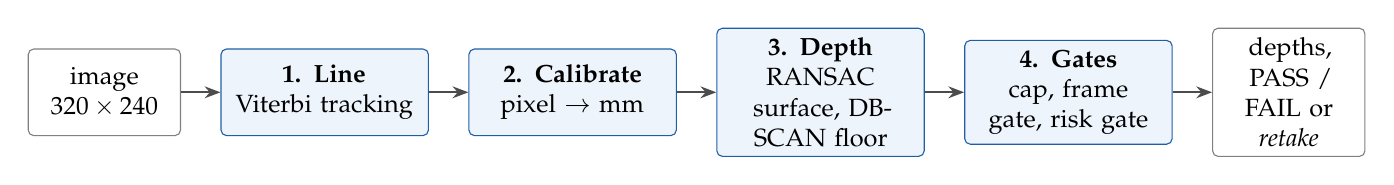
\begin{tikzpicture}[node distance=5mm, every node/.style={font=\small},
  blk/.style={draw=accent, fill=boxbg, rounded corners=2pt, minimum height=11mm, text width=24mm, align=center},
  io/.style={draw=black!50, rounded corners=2pt, minimum height=11mm, text width=17mm, align=center},
  arr/.style={-{Stealth[length=2mm]}, thick, black!70}]
\node[io] (img) {image\\$320\times240$};
\node[blk, right=of img] (dp) {\textbf{1. Line}\\Viterbi tracking};
\node[blk, right=of dp] (cal) {\textbf{2. Calibrate}\\pixel $\to$ mm};
\node[blk, right=of cal] (rd) {\textbf{3. Depth}\\RANSAC surface, DBSCAN floor};
\node[blk, right=of rd] (gate) {\textbf{4. Gates}\\cap, frame gate, risk gate};
\node[io, right=of gate] (out) {depths, PASS / FAIL or \emph{retake}};
\draw[arr] (img)--(dp); \draw[arr] (dp)--(cal); \draw[arr] (cal)--(rd); \draw[arr] (rd)--(gate); \draw[arr] (gate)--(out);
\end{tikzpicture}
\caption{The recommended single-frame pipeline. Stages 1--3 are classical geometry; only the two gates in stage 4
are learned (logistic regression).}
\label{fig:pipeline}
\end{figure}

\begin{lstlisting}[caption={The composition (\texttt{algos/stackcommon.py}, shortened).},label={lst:stack}]
def measure(gray, calib=None, off=None, line_fn=None, cap=False, lb=False, frame_gate=False, risk_model=None):
    line = line_fn(gray, off)                                          # 1. dp_dense.extract_line
    out = robust_depth.stage(line["u"], line["v"], calib, **RD)        # 2. rd_final: floor=dbscan, detect=shape
    out["line"] = line
    if cap:                                                            # 3. deeper than 25 mm is not a groove
        apply_cap(out, gray.shape[0])
    out["verdict"] = verdict_rule(out["grooves"]) if calib is not None else None   # 4. PASS / FAIL / RETAKE
    usable = 1.0 if out["grooves"] else 0.0                            # 5. no groove found = retake
    if frame_gate and usable >= 0.5:                                   #    is there a laser line on a tyre at all?
        out["p_frame"], _ = _prob("frame_lr", gate_features.features(gray)[0])
        usable = min(usable, out["p_frame"])
    if risk_model and calib is not None and usable >= 0.5:             #    is one of these depths probably wrong?
        out["p_bad"], t = _prob(risk_model, stack_features(gray, line, out))
        if out["p_bad"] > t:
            usable = 0.4
    out["usable"] = usable                                             # < 0.5 -> "retake the photo"
    return out
\end{lstlisting}

\subsection{Ablation: what each piece is worth}

Table~\ref{tab:ablation} adds one piece at a time. Rows 1a and 1b each change one thing against the baseline; rows
3--6 build on row 2; row 7 swaps the line extractor of row 2 for laser on/off subtraction.

\begin{table}[H]
\centering\footnotesize\setlength{\tabcolsep}{3.4pt}
\caption{Ablation on \texttt{stress} (top) and on other holder units, \texttt{shifted} (bottom). Depth columns in
mm. Bold = best in column.}\label{tab:ablation}
\begin{tabular}{@{}lrrrrrrrrr@{}}
\toprule
Step & Cov. & MAE & Median & P95 & Gross & Miss & False & Verdict & F.pass \\
\midrule
0\quad Baseline & 1.00 & 1.516 & 0.535 & 6.678 & 0.364 & 0.099 & 0.210 & 0.915 & 0.015 \\
1a\quad DP line only & 1.00 & 0.544 & 0.086 & 0.591 & 0.033 & 0.018 & 0.115 & 0.955 & \textbf{0.000} \\
1b\quad Robust depth only & 1.00 & 0.464 & 0.093 & 2.225 & 0.121 & 0.113 & 0.145 & 0.940 & 0.010 \\
2\quad DP line + robust depth & 1.00 & 0.325 & 0.088 & 0.540 & 0.036 & 0.015 & 0.065 & 0.955 & \textbf{0.000} \\
3\quad + 25 mm cap & 1.00 & 0.325 & 0.088 & 0.540 & 0.036 & 0.015 & 0.065 & 0.955 & \textbf{0.000} \\
4\quad + lower-bound rule & 0.99 & 0.325 & 0.088 & 0.540 & 0.036 & 0.006 & 0.065 & 0.960 & \textbf{0.000} \\
5\quad + risk gate & 0.91 & 0.246 & 0.088 & 0.490 & 0.026 & 0.007 & \textbf{0.016} & \textbf{0.995} & \textbf{0.000} \\
6\quad + frame gate \textbf{(recommended)} & 0.89 & 0.249 & 0.088 & 0.497 & 0.027 & \textbf{0.003} & \textbf{0.017} & \textbf{0.994} & \textbf{0.000} \\
7\quad Row 2 with on/off line & 1.00 & \textbf{0.142} & \textbf{0.084} & \textbf{0.339} & \textbf{0.012} & \textbf{0.003} & 0.025 & 0.975 & 0.005 \\
\bottomrule
\end{tabular}
\\[6pt]
\begin{tabular}{@{}lrrrrrrrrr@{}}
\toprule
Step & Cov. & MAE & Median & P95 & Gross & Miss & False & Verdict & F.pass \\
\midrule
0\quad Baseline & 1.00 & 1.597 & 0.138 & 6.117 & 0.229 & 0.103 & 0.113 & 0.927 & 0.027 \\
1a\quad DP line only & 1.00 & 0.501 & 0.081 & 0.447 & 0.021 & 0.040 & 0.060 & 0.960 & 0.013 \\
1b\quad Robust depth only & 1.00 & 0.479 & 0.056 & 2.133 & 0.082 & 0.087 & 0.093 & 0.960 & \textbf{0.000} \\
2\quad DP line + robust depth & 1.00 & 0.143 & 0.054 & 0.305 & 0.016 & 0.024 & 0.033 & 0.980 & \textbf{0.000} \\
3\quad + 25 mm cap & 1.00 & 0.143 & 0.054 & 0.305 & 0.016 & 0.024 & 0.033 & 0.980 & \textbf{0.000} \\
4\quad + lower-bound rule & 0.99 & 0.143 & 0.054 & 0.305 & 0.016 & 0.020 & 0.034 & 0.986 & \textbf{0.000} \\
5\quad + risk gate & 0.93 & 0.140 & 0.050 & 0.304 & 0.013 & 0.013 & 0.007 & \textbf{1.000} & \textbf{0.000} \\
6\quad + frame gate \textbf{(recommended)} & 0.91 & 0.141 & \textbf{0.048} & 0.305 & 0.013 & 0.013 & 0.007 & \textbf{1.000} & \textbf{0.000} \\
7\quad Row 2 with on/off line & 1.00 & \textbf{0.131} & 0.055 & \textbf{0.238} & \textbf{0.012} & \textbf{0.000} & \textbf{0.000} & \textbf{1.000} & \textbf{0.000} \\
\bottomrule
\end{tabular}

\end{table}

\begin{figure}[H]
\centering
\includegraphics[width=0.92\linewidth]{\figs/best-stack/error_vs_depth.png}
\caption{Depth error of every scored groove, baseline (blue) against the recommended stack (orange), on
\texttt{stress} and \texttt{shifted}. Errors beyond $\pm12$\,mm are clipped to the edge.}
\label{fig:scatter}
\end{figure}

What the table says, in order of importance:
\begin{enumerate}
\item \textbf{A better line and a better depth stage each remove about two thirds of the mean error} (rows 1a, 1b).
      On mean error the two cannot be ranked against each other (Section~\ref{sec:audit}); DP tracking removes more of
      the gross errors (36\,\% $\to$ 3\,\%) and nearly all missed grooves.
\item \textbf{They add up.} Together they reach 0.33\,mm on \texttt{stress} and 0.14\,mm on other
      units, where each alone was near 0.5\,mm. They fix different errors.
\item \textbf{The risk gate buys safety, not accuracy.} For 9\,\% fewer answers it removes three quarters of the
      false grooves and lifts verdict accuracy to 0.995.
\item \textbf{The frame gate} barely changes these sets (every frame shows a tyre); its job is to refuse photos of
      something else (Table~\ref{tab:real}).
\item \textbf{Two ideas did nothing.} The 25\,mm plausibility cap fired on 6 of 1{,}200 training frames. The
      ``lower-bound'' verdict rule (treat a groove with a hidden floor as ``at least $x$\,mm'') never fired on any
      set. Both are kept as harmless safety nets, but neither earned its place on the evidence.
\item \textbf{On/off subtraction would roughly halve the remaining stress error} (row 7) with no gate at all.
\end{enumerate}

\paragraph{What the recommended stack still gets wrong.} On \texttt{stress}, ten grooves carry 56\,\% of all
remaining error; without them the MAE would be 0.11\,mm. All ten are deep grooves (5--17\,mm), so none changes a
PASS/FAIL verdict. Their causes: the floor of a deep groove lost under a dim laser in sunlight (3), paint or
saturation hiding the floor (2), a glint streak inside the groove (3), and geometry such as $2^\circ$ of rocking (2).
\paragraph{Safety in counts.} Rates hide how few illegal tyres the sets contain, so here are counts. Across
\texttt{ideal}, \texttt{stress} and \texttt{shifted} there are 41 illegal tyres: the baseline passed 9 of them, the
recommended stack none. On \texttt{legal} (64 illegal tyres) the baseline passed none and the stack passed one: a
1.58\,mm groove read as 1.60\,mm. The device needs a
\emph{guard band}: PASS only above, say, 1.8\,mm, and ``borderline'' between 1.4 and 1.8\,mm.

\section{Overall comparison}\label{sec:results}

Tables~\ref{tab:stress}--\ref{tab:real} put the main variant of every family side by side. All numbers are generated
from the scorer's JSON output by \texttt{paper/make\_tables.py}; none is typed by hand.

\begin{table}[H]
\centering\footnotesize\setlength{\tabcolsep}{3.4pt}
\caption{\texttt{stress}: 200 simulated frames in bad conditions. Depth columns in mm. Bold = best in column
(the gated rows answer fewer frames, see Cov.).}\label{tab:stress}
\begin{tabular}{@{}llrrrrrrrrrr@{}}
\toprule
Group & Algorithm & Cov. & MAE & Median & P95 & Gross & Miss & False & Verdict & F.pass & CPU ms \\
\midrule
Reference & Baseline (Steger ridge) & 1.00 & 1.516 & 0.535 & 6.678 & 0.364 & 0.099 & 0.210 & 0.915 & 0.015 & 25.8 \\
\addlinespace[2pt]
Per-column peak & Centre of gravity & 1.00 & 1.061 & 0.085 & 8.525 & 0.096 & 0.069 & 0.160 & 0.930 & 0.005 & 18.9 \\
 & 2-D Gaussian + parabola & 1.00 & 1.089 & 0.089 & 5.317 & 0.073 & 0.101 & 0.185 & 0.960 & \textbf{0.000} & 24.1 \\
\addlinespace[2pt]
Tracking & Viterbi line tracking & 1.00 & 0.544 & 0.086 & 0.591 & 0.033 & 0.018 & 0.115 & 0.955 & \textbf{0.000} & 30.6 \\
\addlinespace[2pt]
Learned line & U-Net, augmented & 1.00 & 0.668 & 0.106 & 2.187 & 0.060 & 0.057 & 0.125 & 0.945 & \textbf{0.000} & 67.3 \\
 & U-Net, no augmentation & 1.00 & 0.236 & 0.091 & 0.467 & 0.021 & 0.009 & 0.030 & \textbf{0.985} & \textbf{0.000} & 63.2 \\
 & Candidate classifier (GBM) & 1.00 & 0.273 & 0.088 & 0.561 & 0.024 & 0.024 & 0.020 & 0.970 & \textbf{0.000} & 32.4 \\
\addlinespace[2pt]
Depth stage & Baseline line + robust depth & 1.00 & 0.464 & 0.093 & 2.225 & 0.121 & 0.113 & 0.145 & 0.940 & 0.010 & 37.1 \\
\addlinespace[2pt]
Gate & Baseline + quality gate & 0.16 & \textbf{0.136} & \textbf{0.069} & 0.634 & \textbf{0.000} & 0.107 & 0.031 & 0.906 & 0.005 & 71.3 \\
\addlinespace[2pt]
Two frames & Laser on/off subtraction & 1.00 & 0.147 & 0.080 & \textbf{0.396} & 0.009 & \textbf{0.003} & \textbf{0.010} & 0.980 & \textbf{0.000} & 22.0 \\
\addlinespace[2pt]
No geometry & End-to-end CNN & 1.00 & 0.483 & 0.247 & 1.963 & 0.102 & 0.006 & 0.015 & 0.980 & 0.015 & 2.3 \\
\bottomrule
\end{tabular}

\end{table}

\begin{table}[H]
\centering\footnotesize\setlength{\tabcolsep}{3.4pt}
\caption{\texttt{ideal}: 150 simulated frames with the holder locked on a clean tyre.}\label{tab:ideal}
\begin{tabular}{@{}llrrrrrrrrrr@{}}
\toprule
Group & Algorithm & Cov. & MAE & Median & P95 & Gross & Miss & False & Verdict & F.pass & CPU ms \\
\midrule
Reference & Baseline (Steger ridge) & 1.00 & 0.147 & 0.054 & 0.474 & 0.008 & 0.090 & \textbf{0.000} & 0.980 & 0.013 & 28.1 \\
\addlinespace[2pt]
Per-column peak & Centre of gravity & 1.00 & 0.062 & 0.039 & 0.191 & \textbf{0.000} & 0.030 & \textbf{0.000} & 0.987 & 0.013 & 20.2 \\
 & 2-D Gaussian + parabola & 1.00 & 0.060 & 0.039 & 0.176 & \textbf{0.000} & 0.041 & \textbf{0.000} & 0.987 & 0.013 & 20.9 \\
\addlinespace[2pt]
Tracking & Viterbi line tracking & 1.00 & 0.064 & 0.041 & 0.186 & \textbf{0.000} & 0.015 & \textbf{0.000} & 0.987 & 0.013 & 27.5 \\
\addlinespace[2pt]
Learned line & U-Net, augmented & 1.00 & 0.061 & 0.040 & 0.173 & \textbf{0.000} & 0.019 & \textbf{0.000} & 0.987 & 0.013 & 63.9 \\
 & U-Net, no augmentation & 1.00 & 0.055 & 0.032 & 0.156 & \textbf{0.000} & 0.011 & \textbf{0.000} & 0.987 & 0.013 & 56.7 \\
 & Candidate classifier (GBM) & 1.00 & 0.154 & 0.079 & 0.527 & \textbf{0.000} & 0.015 & \textbf{0.000} & 0.987 & 0.013 & 32.1 \\
\addlinespace[2pt]
Depth stage & Baseline line + robust depth & 1.00 & 0.081 & \textbf{0.022} & 0.157 & 0.004 & 0.082 & \textbf{0.000} & 0.987 & \textbf{0.000} & 37.0 \\
\addlinespace[2pt]
Gate & Baseline + quality gate & 0.88 & 0.107 & 0.048 & 0.433 & 0.005 & 0.080 & \textbf{0.000} & 0.985 & 0.013 & 72.8 \\
\addlinespace[2pt]
Two frames & Laser on/off subtraction & 1.00 & 0.062 & 0.037 & 0.192 & \textbf{0.000} & 0.015 & \textbf{0.000} & 0.987 & 0.013 & 18.5 \\
\addlinespace[2pt]
No geometry & End-to-end CNN & 1.00 & 0.100 & 0.074 & 0.277 & \textbf{0.000} & \textbf{0.000} & \textbf{0.000} & \textbf{1.000} & \textbf{0.000} & 2.3 \\
\addlinespace[2pt]
Combined & DP line + robust depth & 1.00 & 0.039 & 0.027 & 0.102 & \textbf{0.000} & \textbf{0.000} & \textbf{0.000} & \textbf{1.000} & \textbf{0.000} & 37.7 \\
 & \textbf{Recommended stack} (+ gates) & 1.00 & 0.039 & 0.027 & 0.102 & \textbf{0.000} & \textbf{0.000} & \textbf{0.000} & \textbf{1.000} & \textbf{0.000} & 102.8 \\
 & On/off line + robust depth & 1.00 & \textbf{0.030} & \textbf{0.022} & \textbf{0.085} & \textbf{0.000} & \textbf{0.000} & \textbf{0.000} & \textbf{1.000} & \textbf{0.000} & 28.3 \\
\bottomrule
\end{tabular}

\end{table}

\begin{table}[H]
\centering\footnotesize\setlength{\tabcolsep}{3.4pt}
\caption{\texttt{legal}: 150 worn tyres around the 1.6\,mm limit. Here F.pass is the number that matters.}\label{tab:legal}
\begin{tabular}{@{}llrrrrrrrrrr@{}}
\toprule
Group & Algorithm & Cov. & MAE & Median & P95 & Gross & Miss & False & Verdict & F.pass & CPU ms \\
\midrule
Reference & Baseline (Steger ridge) & 1.00 & 0.053 & 0.030 & 0.210 & \textbf{0.000} & 0.054 & \textbf{0.000} & \textbf{0.993} & \textbf{0.000} & 25.8 \\
\addlinespace[2pt]
Per-column peak & Centre of gravity & 1.00 & 0.024 & 0.019 & 0.064 & \textbf{0.000} & 0.054 & \textbf{0.000} & \textbf{0.993} & \textbf{0.000} & 20.8 \\
 & 2-D Gaussian + parabola & 1.00 & 0.029 & 0.025 & 0.068 & \textbf{0.000} & 0.054 & \textbf{0.000} & \textbf{0.993} & \textbf{0.000} & 22.8 \\
\addlinespace[2pt]
Tracking & Viterbi line tracking & 1.00 & 0.032 & 0.026 & 0.072 & \textbf{0.000} & 0.051 & \textbf{0.000} & \textbf{0.993} & \textbf{0.000} & 27.9 \\
\addlinespace[2pt]
Learned line & U-Net, augmented & 1.00 & 0.036 & 0.033 & 0.087 & \textbf{0.000} & 0.054 & \textbf{0.000} & 0.987 & 0.007 & 62.8 \\
 & U-Net, no augmentation & 1.00 & 0.035 & 0.025 & 0.079 & \textbf{0.000} & 0.054 & \textbf{0.000} & \textbf{0.993} & \textbf{0.000} & 60.1 \\
 & Candidate classifier (GBM) & 1.00 & 0.044 & 0.028 & 0.083 & \textbf{0.000} & 0.051 & \textbf{0.000} & 0.987 & \textbf{0.000} & 25.0 \\
\addlinespace[2pt]
Depth stage & Baseline line + robust depth & 1.00 & \textbf{0.019} & 0.016 & \textbf{0.047} & \textbf{0.000} & \textbf{0.000} & \textbf{0.000} & \textbf{0.993} & \textbf{0.000} & 37.5 \\
\addlinespace[2pt]
Gate & Baseline + quality gate & 0.96 & 0.053 & 0.030 & 0.212 & \textbf{0.000} & 0.035 & \textbf{0.000} & \textbf{0.993} & \textbf{0.000} & 77.4 \\
\addlinespace[2pt]
Two frames & Laser on/off subtraction & 1.00 & 0.026 & 0.020 & 0.066 & \textbf{0.000} & 0.054 & \textbf{0.000} & 0.987 & 0.007 & 22.7 \\
\addlinespace[2pt]
No geometry & End-to-end CNN & 1.00 & 0.072 & 0.062 & 0.187 & \textbf{0.000} & 0.003 & \textbf{0.000} & 0.967 & 0.027 & 2.3 \\
\addlinespace[2pt]
Combined & DP line + robust depth & 1.00 & 0.024 & 0.019 & 0.061 & \textbf{0.000} & \textbf{0.000} & \textbf{0.000} & 0.987 & 0.007 & 39.4 \\
 & \textbf{Recommended stack} (+ gates) & 1.00 & 0.024 & 0.019 & 0.061 & \textbf{0.000} & \textbf{0.000} & \textbf{0.000} & 0.987 & 0.007 & 101.2 \\
 & On/off line + robust depth & 1.00 & \textbf{0.019} & \textbf{0.014} & 0.051 & \textbf{0.000} & \textbf{0.000} & \textbf{0.000} & \textbf{0.993} & \textbf{0.000} & 30.5 \\
\bottomrule
\end{tabular}

\end{table}

\begin{table}[H]
\centering\footnotesize\setlength{\tabcolsep}{3.4pt}
\caption{\texttt{shifted}: three other holder units, each with its own calibration.}\label{tab:shifted}
\begin{tabular}{@{}llrrrrrrrrrr@{}}
\toprule
Group & Algorithm & Cov. & MAE & Median & P95 & Gross & Miss & False & Verdict & F.pass & CPU ms \\
\midrule
Reference & Baseline (Steger ridge) & 1.00 & 1.597 & 0.138 & 6.117 & 0.229 & 0.103 & 0.113 & 0.927 & 0.027 & 24.7 \\
\addlinespace[2pt]
Per-column peak & Centre of gravity & 1.00 & 1.199 & 0.077 & 8.984 & 0.095 & 0.087 & 0.187 & 0.907 & 0.027 & 19.3 \\
 & 2-D Gaussian + parabola & 1.00 & 1.059 & 0.075 & 7.237 & 0.095 & 0.123 & 0.180 & 0.907 & 0.027 & 21.2 \\
\addlinespace[2pt]
Tracking & Viterbi line tracking & 1.00 & 0.501 & 0.081 & 0.447 & 0.021 & 0.040 & 0.060 & 0.960 & 0.013 & 30.5 \\
\addlinespace[2pt]
Learned line & U-Net, augmented & 1.00 & 0.416 & 0.071 & 0.567 & 0.047 & 0.079 & 0.093 & 0.940 & 0.020 & 62.9 \\
 & U-Net, no augmentation & 1.00 & 0.132 & 0.065 & \textbf{0.358} & 0.016 & \textbf{0.028} & 0.047 & 0.973 & 0.013 & 63.0 \\
 & Candidate classifier (GBM) & 1.00 & 0.466 & 0.093 & 1.766 & 0.066 & 0.040 & 0.047 & 0.953 & 0.020 & 29.0 \\
\addlinespace[2pt]
Depth stage & Baseline line + robust depth & 1.00 & 0.479 & \textbf{0.056} & 2.133 & 0.082 & 0.087 & 0.093 & 0.960 & \textbf{0.000} & 35.1 \\
\addlinespace[2pt]
Gate & Baseline + quality gate & 0.52 & \textbf{0.117} & 0.067 & 0.414 & \textbf{0.000} & 0.073 & \textbf{0.000} & \textbf{0.987} & 0.007 & 63.8 \\
\addlinespace[2pt]
Two frames & Laser on/off subtraction & 1.00 & 0.182 & 0.073 & 0.383 & 0.008 & \textbf{0.028} & \textbf{0.000} & 0.987 & 0.013 & 22.3 \\
\addlinespace[2pt]
No geometry & End-to-end CNN & 1.00 & 5.216 & 3.231 & 19.888 & 0.754 & 0.115 & 1.953 & 0.907 & 0.087 & 2.7 \\
\bottomrule
\end{tabular}

\end{table}

\begin{table}[H]
\centering\footnotesize\setlength{\tabcolsep}{3.4pt}
\caption{\texttt{handheld}: 150 simulated frames built to resemble the real photos; errors in pixels of line shift.
The end-to-end network outputs millimetres only and cannot be scored here.}\label{tab:handheld}
\begin{tabular}{@{}llrrrrrrr@{}}
\toprule
Group & Algorithm & Cov. & Line F1 & MAE px & Median px & Gross & Miss & False \\
\midrule
Reference & Baseline (Steger ridge) & 1.00 & 0.385 & 8.11 & 2.81 & 0.494 & 0.466 & 0.327 \\
\addlinespace[2pt]
Per-column peak & Centre of gravity & 1.00 & 0.757 & 2.94 & 0.54 & 0.196 & 0.061 & 0.740 \\
 & 2-D Gaussian + parabola & 1.00 & 0.841 & 2.63 & 0.51 & 0.127 & 0.080 & 0.427 \\
\addlinespace[2pt]
Tracking & Viterbi line tracking & 1.00 & \textbf{0.905} & 3.66 & \textbf{0.40} & 0.103 & \textbf{0.043} & 0.233 \\
\addlinespace[2pt]
Learned line & U-Net, augmented & 1.00 & 0.903 & 1.63 & 0.56 & 0.077 & 0.049 & 0.047 \\
 & U-Net, no augmentation & 1.00 & 0.744 & 1.55 & 0.69 & 0.115 & 0.092 & 0.253 \\
 & Candidate classifier (GBM) & 1.00 & 0.516 & 1.87 & 0.45 & 0.133 & 0.632 & 0.007 \\
\addlinespace[2pt]
Depth stage & Baseline line + robust depth & 1.00 & 0.385 & 7.06 & 0.61 & 0.354 & 0.515 & 0.300 \\
\addlinespace[2pt]
Gate & Baseline + quality gate & 0.34 & 0.785 & 3.77 & 1.96 & 0.294 & 0.056 & 0.196 \\
\addlinespace[2pt]
Two frames & Laser on/off subtraction & 1.00 & 0.753 & \textbf{1.11} & 0.56 & \textbf{0.045} & \textbf{0.043} & 0.453 \\
\addlinespace[2pt]
No geometry & End-to-end CNN & 0.99 & -- & -- & -- & -- & 1.000 & \textbf{0.000} \\
\bottomrule
\end{tabular}

\end{table}

\begin{table}[H]
\centering\footnotesize\setlength{\tabcolsep}{3.4pt}
\caption{Real photos (86). ``$\Delta$\,px'' is the mean difference from the baseline-derived reference on six
truck-tyre frames, so the baseline's own row is near zero by construction. ``Usable kept'': share of the 19 good
photos answered. ``F.meas'': share of unusable photos on which a depth was still reported (55 with no laser,
12 with a laser that cannot be measured). The gate rows are in-sample for the frame gate; cross-validated values
are in the text. Methods needing a laser-off frame or a calibration are omitted.}\label{tab:real}
\begin{tabular}{@{}llrrrrrrr@{}}
\toprule
Group & Algorithm & Line F1 & $\Delta$ px & Found & Within 3 px & Usable kept & F.meas (no laser) & F.meas (laser) \\
\midrule
Reference & Baseline (Steger ridge) & \textbf{1.000} & 0.13 & 6/6 & 6/6 & \textbf{0.947} & 0.691 & 0.750 \\
\addlinespace[2pt]
Per-column peak & Centre of gravity & 0.891 & 5.11 & 5/6 & 3/6 & 0.789 & 0.709 & 0.667 \\
 & 2-D Gaussian + parabola & 0.926 & 1.14 & 6/6 & 5/6 & 0.895 & 0.818 & 0.667 \\
\addlinespace[2pt]
Tracking & Viterbi line tracking & 0.943 & 1.13 & 6/6 & 5/6 & 0.842 & 0.545 & 0.833 \\
\addlinespace[2pt]
Learned line & U-Net, augmented & 0.920 & 1.08 & 6/6 & 5/6 & 0.895 & 0.455 & 0.667 \\
 & U-Net, no augmentation & 0.895 & 7.15 & 6/6 & 3/6 & 0.895 & 0.455 & 0.333 \\
 & Candidate classifier (GBM) & 0.869 & 10.93 & 2/6 & 1/6 & 0.579 & 0.473 & \textbf{0.083} \\
\addlinespace[2pt]
Depth stage & Baseline line + robust depth & \textbf{1.000} & 1.19 & 6/6 & 6/6 & \textbf{0.947} & 0.636 & 0.583 \\
\addlinespace[2pt]
Gate & Baseline + quality gate & \textbf{1.000} & 0.13 & 6/6 & 6/6 & 0.895 & 0.036 & 0.250 \\
\addlinespace[2pt]
Combined & DP line + robust depth & 0.943 & 0.95 & 6/6 & 6/6 & 0.842 & 0.545 & 0.833 \\
 & \textbf{Recommended stack} (+ gates) & 0.943 & 0.95 & 6/6 & 6/6 & 0.789 & \textbf{0.018} & 0.250 \\
\bottomrule
\end{tabular}

\end{table}

\begin{figure}[H]
\centering
\includegraphics[width=0.88\linewidth]{\figs/best-stack/real_overlay.png}
\caption{Baseline (blue) and recommended (orange) lines on three real photos. On the truck tyre they agree to within
a pixel. On the cluttered rover photo both follow background edges; this is the kind of frame the gate must refuse.}
\label{fig:realoverlay}
\end{figure}

\paragraph{Reading the real-photo table.} Three things can be said. First, the recommended stack agrees with the
reference to about 1\,px on all six truck frames, which at the holder's scale would be about 0.5\,mm; whether the
stack or the reference is nearer the truth is unknown. Second, without a gate \emph{every} method reports depths on
half or more of the photos that show no laser at all. Third, with the gate, and with the frame gate re-fitted
without the photos being scored (leave-one-session-out), the stack answers 15 of 19 usable photos, 0 of 55 photos
with no laser, and 3 of 12 photos with an unusable laser.

\section{Preliminary hand-held test against a known depth}\label{sec:prelim}

\caution{\textbf{This section is a preliminary testing stage.} The photos were taken by hand, \emph{without} the
printed holder, with the laser not fixed to the camera and with no calibration. It is included as a first
comparison against a real depth, not as a measure of the device's accuracy.}

The truck tyre photographed on 30 October has a tread depth of about 9\,mm (the team's own manual measurement).
Table~\ref{tab:prelim} compares that with what the recommended pipeline reports on the photos of that tyre it
accepted, using \texttt{research/session.py}. Without a calibration, pixels are converted to millimetres with the
\emph{design} geometry: laser at $35^\circ$ and the camera 90\,mm from the tread.

\begin{table}[H]
\centering\small
\caption{Preliminary hand-held test, truck tyre, true depth about 9\,mm. ``Range'' is the same pixel reading
converted at 70 and at 110\,mm stand-off.}\label{tab:prelim}
\begin{tabular}{@{}lrrrr@{}}
\toprule
Photo (30 Oct) & Line shift (px) & At 90\,mm (mm) & Range (mm) & Estimate / true \\
\midrule
\texttt{154820} & 34.3 & 21.9 & 12.6--34.7 & 2.4$\times$ \\
\texttt{154854} (same spot) & 36.6 & 23.8 & 13.6--37.8 & 2.6$\times$ \\
\texttt{154554} & 46.3 & 32.4 & 18.2--52.6 & 3.6$\times$ \\
\texttt{154510} & 52.1 & 38.1 & 21.1--62.9 & 4.2$\times$ \\
\midrule
\texttt{154700}, \texttt{154748}, \texttt{154813} & 75--93 & 67--101 & -- & 7--11$\times$ \\
\bottomrule
\end{tabular}
\end{table}

\paragraph{What this shows.}
\begin{itemize}
\item \textbf{The pixel measurement repeats.} Two presses on the same spot give 34.3 and 36.6\,px, about 6\,\% apart.
\item \textbf{The millimetre values are 2.4 to 4.2 times too large.} At the design geometry a 9\,mm groove should shift
      the line by about 16\,px; the photos show 34--52\,px. That is what a camera held only 50--60\,mm from the
      tread would give, or a laser held at a steeper angle, or both. With a hand-held, unfixed laser the two cannot
      be told apart, and the scale changes from photo to photo (3.8 to 5.8\,px per mm here).
\item \textbf{Three readings are not groove floors at all.} Shifts of 75--93\,px are the line tracker following
      something else, and the gate accepted them. In pixel mode the 25\,mm plausibility cap cannot act, because
      without a calibration the software does not know what 25\,mm is.
\end{itemize}

\paragraph{What it means.} This test says nothing against the line finding and nothing for the accuracy: the
conversion from pixels to millimetres depends on a geometry that was not fixed. It is the practical case for the
holder. Depth error grows with the square of the stand-off error, so a rigid camera--laser mount at a known height,
followed by a shim calibration, is required before any millimetre value can be trusted. Until then the software
should report pixels, and its millimetre column should be read as a rough indication only.

\paragraph{Positioning lessons for the next session.} Fix the laser to the camera; keep a constant stand-off;
look straight down with the laser line crossing the grooves at a right angle; centre the groove of interest;
measure on a straight section of groove, away from zig-zag corners and wear-indicator bars; and lower the
exposure until the laser line is thin rather than a saturated band.

\section{Discussion}\label{sec:discussion}

\paragraph{Where the error came from.} Before this study we assumed the weak point was sub-pixel accuracy. It is
not. On clean frames every method is within 0.03--0.15\,mm. The baseline's large stress errors come from three
specific faults, each with a specific classical fix: (i) no notion of ``one line'' (fixed by DP tracking), (ii) a
depth stage that fits in image columns and lets one stray point set the floor (fixed by fitting in millimetres and
clustering the floor), and (iii) no ability to say ``retake'' (fixed by the gate).

\paragraph{Classical or learned?} Table~\ref{tab:verdicts} summarises each family. The pattern is consistent:
learned methods looked best on the simulated sets that resemble their training data and lost most when the
pictures changed (another unit, a hand-held photo). The classical methods moved least. Learning earned its place in
one role: the small logistic-regression gates, where the question is fuzzy (``does this look like a usable photo?'')
and a wrong answer costs a retake rather than a wrong measurement.

\begin{table}[H]
\centering\small
\caption{Summary verdict per family.}\label{tab:verdicts}
\begin{tabularx}{\linewidth}{@{}lllX@{}}
\toprule
Family & Simulation & Real photos & Verdict \\
\midrule
DP line tracking & strong & agrees ($\approx$1\,px) & \textbf{Adopt} as the line extractor. \\
Robust depth stage & strong & consistent on the repeat pair & \textbf{Adopt}. Confirm against a gauge. \\
Quality gate & strong & 0.24 false-accept, cross-validated & \textbf{Adopt}; retrain as labelled sessions grow. \\
Calibration (physical model) & strong & not testable yet & \textbf{Adopt} the eight-height recipe and zero check. \\
Laser on/off & best of all & needs hardware & \textbf{Hardware request}: laser on a GPIO. \\
Per-column peaks & accurate, fragile & mixed & Keep as the fast option if the MCU budget is tight. \\
U-Net line & strong & agrees ($\approx$1\,px) & Park until real holder images exist. \\
Candidate classifier & strong & fails & Do not use: learned a simulator shortcut. \\
End-to-end CNN & good in-domain & fails & Do not use as the measurement. \\
\bottomrule
\end{tabularx}
\end{table}

\paragraph{Computing cost.} On one laptop-class core the recommended stack without the frame gate takes about
35--40\,ms per frame, against about 26\,ms for the baseline; the frame gate's features roughly double that and are
the first thing to optimise. Timings on the shared test machine varied by $\pm30\,\%$ between runs, so treat them as
rough. Nothing in stages 1--3 needs more than NumPy-style array operations, so a port to the STM32H7 or to the
cloud back-end is realistic; the U-Net is not realistic on the microcontroller.

\section{Independent audit}\label{sec:audit}

Before writing this report, a separate reviewer that had written none of the code re-ran the key results from a
clean checkout and looked for mistakes. The full audit is in \texttt{research/audit/AUDIT.md}; Table~\ref{tab:audit}
summarises it.

\begin{table}[H]
\centering\small
\caption{Audit summary.}\label{tab:audit}
\begin{tabularx}{\linewidth}{@{}lX@{}}
\toprule
Check & Outcome \\
\midrule
Reproducibility & Nine algorithms re-scored; every one of 89 metrics per algorithm matched the stored value exactly. \\
Data integrity & Test frames regenerate bit-for-bit from their seeds; the six simulated sets share no scenes. \\
Leakage & No learned model was trained or tuned on a test set. One in-sample number: the frame gate on real photos
          (flagged wherever it appears). \\
Scorer & Behaves correctly on synthetic perfect, empty and always-abstain algorithms. Three quirks found (below). \\
\bottomrule
\end{tabularx}
\end{table}

\paragraph{What the audit changed in this report.}
\begin{itemize}
\item \textbf{Means have wide error bars.} A few gross failures dominate every stress MAE: for DP tracking, seven
      grooves carry 78\,\% of the total error. Table~\ref{tab:boot} gives bootstrap intervals. Both improvements over
      the baseline are real; DP tracking and the robust depth stage \emph{cannot be ranked against each other} on
      mean error. We therefore report medians and gross-error rates next to every mean, and we do not rank the
      better methods by small MAE differences.
\item \textbf{Unsafe-PASS rates rest on few tyres.} Only 10, 17 and 14 tyres are illegal in \texttt{ideal},
      \texttt{stress} and \texttt{shifted}; ``0.000'' there means ``0 of 17''. Counts are given in
      Section~\ref{sec:stack}. Verdict accuracy on those sets is also flattering: always answering PASS would score
      0.915 on \texttt{stress}. Only \texttt{legal} (64 illegal tyres of 150) supports a verdict claim.
\item \textbf{A scoring artefact was removed.} The scorer showed the end-to-end network making no false measurements
      on real photos, because it outputs millimetres and the real-photo scorer only counts pixel outputs. Run
      directly, it reports a depth on 43 of 67 unusable photos. Its rows are left out of the real and hand-held
      tables.
\item \textbf{On/off numbers are for a perfectly still device.} In the benchmark the laser-off frame is the same
      scene with no motion. The effect of motion was studied separately (Figure~\ref{fig:onoff}), and there is no
      real-photo evidence for on/off at all.
\item \textbf{The U-Net was trained once}, with one random seed; its numbers have unknown run-to-run spread.
\end{itemize}

\begin{table}[H]
\centering\small
\caption{Bootstrap over frames (1{,}000 resamples) on \texttt{stress}: depth error in mm with 95\,\% intervals.}\label{tab:boot}
\begin{tabular}{@{}lllrr@{}}
\toprule
Algorithm & MAE [95\,\% interval] & Median [95\,\% interval] & Error carried by worst 5\,\% & MAE without them \\
\midrule
Baseline & 1.52 [1.13, 1.93] & 0.54 [0.32, 0.67] & 48\,\% & 0.83 \\
DP line only & 0.54 [0.25, 0.94] & 0.09 [0.07, 0.11] & 78\,\% & 0.12 \\
Robust depth only & 0.46 [0.34, 0.63] & 0.09 [0.07, 0.11] & 53\,\% & 0.23 \\
\midrule
\multicolumn{5}{@{}l}{Paired differences in MAE: baseline $-$ DP $=0.95$ [0.44, 1.45]; baseline $-$ robust depth $=1.03$ [0.68, 1.45];}\\
\multicolumn{5}{@{}l}{DP $-$ robust depth $=0.08$ [$-0.24$, $+0.48$] (no detectable difference).}\\
\bottomrule
\end{tabular}
\end{table}


\section{Threats to validity}\label{sec:validity}

We list these plainly because they decide how far the numbers above can be trusted.

\begin{enumerate}
\item \textbf{Most numbers come from a simulator.} It models geometry, blur, noise, glints and dirt, but its line is
      thinner than the real one, always sits at the same height in the frame in the standard sets, and its tread
      crown is an exact parabola. Two learned methods exploited such regularities. The \texttt{handheld} and
      \texttt{shifted} sets were added to expose this, but they are still simulations.
\item \textbf{The simulator shares assumptions with some methods.} Its camera is exactly the physical calibration
      model, and its crown is exactly what the robust depth stage fits. Gains in those two places are upper bounds.
\item \textbf{The real photos were not taken with the holder.} They are hand-held, the laser was not fixed to the
      camera, and no groove was measured with a gauge. Their depths are meaningful only in pixels, and the six
      reference depths come from the baseline itself. Six frames cannot rank methods that differ by a pixel.
\item \textbf{Small numbers.} 19 usable photos, 12 with an unusable laser. One photo is 5--8 percentage points.
\item \textbf{In-sample gate numbers.} The frame gate was trained on the same 86 photos; we quote cross-validated
      figures wherever we draw a conclusion. All 19 usable photos come from two sessions, so even those are a
      feasibility result rather than a performance estimate.
\item \textbf{Tuning.} All thresholds were tuned on \texttt{train}. Two choices in the combined stack were made
      after test numbers had been seen (the pixel cap, and the 3\,\% risk target); neither changes a conclusion.
\item \textbf{Scorer limits.} There is no ``at least $x$\,mm'' outcome and no guard band at 1.6\,mm, so a 0.02\,mm
      slip across the limit counts the same as a gross unsafe PASS; verdict accuracy is also inflated by the fact
      that most simulated tyres are legal.
\end{enumerate}

\section{Recommendations and next steps}

\paragraph{Software (ready now).}
\begin{enumerate}
\item Replace the Steger line extractor with \algo{dp\_dense} and the depth stage with \algo{rd\_final}; add the
      gates. This is \algo{stack\_dp\_rd\_gate} on branch \texttt{research/best-stack}.
\item Report three outcomes, not two: PASS, FAIL, and \emph{retake}. Add a guard band around 1.6\,mm.
\item Switch calibration to the physical model with eight plate heights from $+4$ to $-18$\,mm, and add a
      one-photo zero check at the start of a shift.
\end{enumerate}

\paragraph{Hardware (one request).} Let the microcontroller switch the laser, and capture an off frame within a
few milliseconds of the on frame. In simulation this is worth more than any other single change.

\paragraph{Data (the real gap).} Everything above should be confirmed on images from the printed holder:
\begin{enumerate}
\item With the holder, photograph 5--10 tyres, three presses per groove, and measure each groove with the manual
      gauge. Fifty gauge readings would turn every ``agreement'' number in this report into an accuracy number.
\item Photograph a machined step block (for example 2, 5 and 10\,mm steps) to check the calibration end to end.
\item Keep labelling ``usable / not usable'' on every session; the gate improves with sessions, not with model size.
\end{enumerate}

\section{Conclusion}

Ten algorithm families were implemented on separate branches and scored on the same simulated and real data.
The most effective changes were not the most sophisticated ones: a dynamic-programming line tracker, a depth stage
that works in millimetres and takes the groove floor from a cluster, and a small gate that can refuse a photo.
In simulation, together they cut the mean depth error under bad conditions from 1.5\,mm to 0.25\,mm, cut gross errors
from 36\,\% to under 3\,\%, passed none of 41 illegal tyres where the baseline passed 9, and stopped the device from reporting
depths on photos with no laser, while still answering about nine presses in ten. Neural networks that replace the
geometry looked good in simulation and failed on real photos and on other units. The next step is not a better
algorithm but ground truth: gauge-measured grooves photographed through the printed holder.

\appendix
\section{Reproducing the results}

\begin{lstlisting}[language=bash]
git clone https://github.com/Advait-B/urex && cd urex
git checkout research/paper                 # everything merged: simulator, benchmark, all algorithms, this paper
pip install numpy scipy scikit-learn scikit-image opencv-python-headless torch
cd research
python -m bench.run2 algos.stack_dp_rd_gate --out results2/stack_dp_rd_gate.json   # score one algorithm
python -m bench.score_all algos.dp_dense algos.rd_final                             # re-score several
python paper/make_tables.py && (cd paper && pdflatex main.tex)                      # rebuild tables and PDF
\end{lstlisting}

The simulated sets are generated from fixed seeds the first time they are needed (a few minutes) and cached.
Each branch has a write-up in \texttt{research/notes/<topic>.md} with more variants, figures and negative results
than fit here.

\end{document}
